\begin{figure*}
    \begin{subfigure}{.333\textwidth}
        \centering
        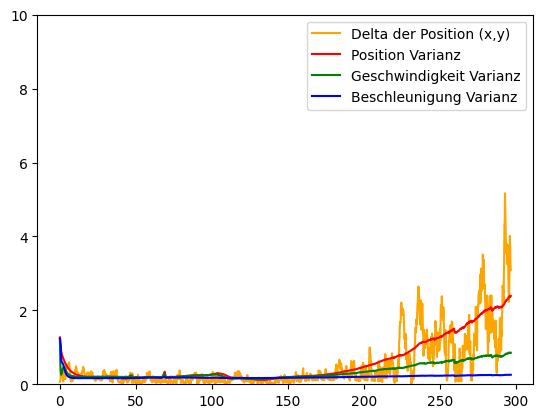
\includegraphics[width=.9\linewidth]{Ergebnisse/plots_ungenauigkeiten/winkel/winkel_const_vel_basic.png}  
        \caption{Optimale Simulationsbedinungen}
        % \label{}
    \end{subfigure}    
    \begin{subfigure}{.333\textwidth}
        \centering
        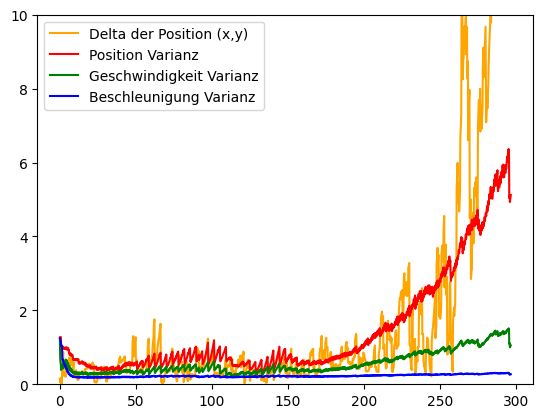
\includegraphics[width=.9\linewidth]{Ergebnisse/plots_ungenauigkeiten/winkel/winkel_const_vel_freq.png}  
        \caption{Türme unterschiedlich frequent}
    \end{subfigure}    
    \begin{subfigure}{.333\textwidth}
        \centering
        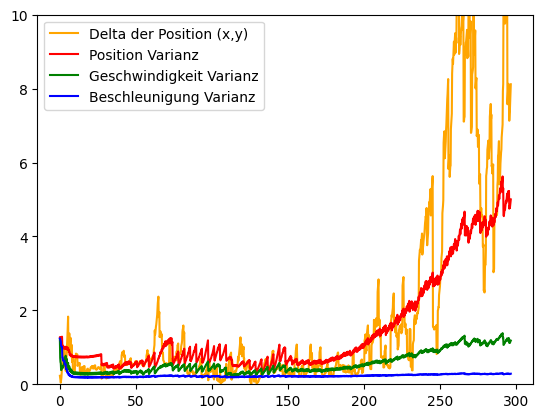
\includegraphics[width=.9\linewidth]{Ergebnisse/plots_ungenauigkeiten/winkel/winkel_const_vel_flag_freq.png}
        \caption{Türme unterschiedlich frequent, ausfallend}
    \end{subfigure}
    \caption{Winkelansatz: Fehler und Varianzen bei konstanter Geschwindigkeit}
    \label{abb:winkel-cv-fehler}
\end{figure*}
